\section{Dinámicas especiales}

\subsection{Canales de Pauli}

Los canales de Pauli son canales cuánticos en los que se aplica un operador de Pauli con alguna probabilidad. El canal de Pauli de un qubit más general está definido como
\begin{gather}
    P:\mcB(\hilbert_{2}) \rightarrow \mcB(\hilbert_{2})\nonumber\\
    P(\Delta)=\sum_{j=0}^{3}q_{j}\pauli{j}\Delta\pauli{j}\,\text{ con }\, \sum_{j=0}^{3}q_{j}=1\rlap{.}\nonumber
\end{gather}
Reconociendo que cualquiera de los tres operadores de Pauli puede escribirse en términos de los otros dos, se puede aprovechar la relación $-i\pauli{2}=\pauli{1}\pauli{3}$ para escribir a los canales de Pauli de una forma particularmente útil:
\begin{equation}
    P(\Delta)=\sum_{j,k=0}^{1}q_{j,k}\pauli{1}^{j}\pauli{3}^{k}\Delta\pauli{3}^{k}\pauli{1}^{j}.\nonumber
\end{equation}
A través de esta expresión se extienden los canales de Pauli de un qubit a $n$ qubits como \acnote{agregar cita}
\begin{gather}\label{eq:PauliChannelN}
    P:\mcB(\hilbert_{2^{n}}) \rightarrow \mcB(\hilbert_{2^{n}})\nonumber\\
    P(\Delta)=\sum_{\vec{j},\vec{k}}q_{\vec{j},\vec{k}}\pauli{1}^{\vec{j}}\pauli{3}^{\vec{k}}\Delta\pauli{3}^{\vec{k}}\pauli{1}^{\vec{j}}\rlap{.}
\end{gather}
donde $\pauli{j}^{\vec{k}}=\pauli{j}^{k_{1}}\otimes\pauli{j}^{k_{2}}\otimes ... \otimes \pauli{j}^{k_{n}}$ y las entradas $k_{l}$ del vector $\vec{k}$ solo pueden valer $0$ o $1$.

\subsubsection{Canales de desfasamiento}

Por canales de desfasamiento se entiende aquellos canales cuánticos cuyo efecto es amortiguar los elementos fuera de la diagonal del operador sobre el que actúan. A notar que esta definición es dependiente de la base sobre la que se está trabajando. Por ejemplo, sea $\rho\in\densityspace{2}$. Si se utiliza la base de eigenestados de $\pauli{3}$, entonces el canal
\begin{equation}
    \rho\mapsto q_{1}\rho + q_{2} \pauli{3}\rho\pauli{3}\nonumber
\end{equation}
es un canal de desfasamiento. En efecto, la acción de este canal sobre los elementos de matriz de $\rho$ es
\begin{equation}
    \begin{pmatrix}
        \rho_{0,0} & \rho_{0,1}\\
        \rho_{1,0} & \rho_{1,1}\\
    \end{pmatrix}\mapsto\begin{pmatrix}
        \rho_{0,0} & (q_{1}-q_{2})\rho_{0,1}\\
        (q_{1}-q_{2})\rho_{1,0} & \rho_{1,1}\\
    \end{pmatrix},\nonumber
\end{equation}
mientras que el canal de \textit{bit flip},
\begin{equation}
    \rho\mapsto q_{1}\rho + q_{2} \pauli{1}\rho\pauli{1},\nonumber
\end{equation}
no lo es, pues su acción sobre los elementos de matriz de $\rho$ es
\begin{equation}
    \begin{pmatrix}
        \rho_{0,0} & \rho_{0,1}\\
        \rho_{1,0} & \rho_{1,1}\\
    \end{pmatrix}\mapsto\begin{pmatrix}
        \frac{1}{2}\qty(1+(q_{1}-q_{2})(2\rho_{0,0}-1)) & \Re(\rho_{0,1})-\rmi(q_{1}-q_{2})\Im(\rho_{0,1})\\
        \Re(\rho_{1,0})+\rmi(q_{1}-q_{2})\Im(\rho_{1,0}) & \frac{1}{2}\qty(1-(q_{1}-q_{2})(1-2\rho_{1,1}))\\
    \end{pmatrix}.\nonumber
\end{equation}
Por supuesto, el canal de \textit{bit flip} es un canal de desfasamiento si se trabaja en la base de los eigenestados de $\pauli{1}$, pues en esta base, la acción del canal de \textit{bit flip} es
\begin{equation}
    \begin{pmatrix}
        \rho_{0,0} & \rho_{0,1}\\
        \rho_{1,0} & \rho_{1,1}\\
    \end{pmatrix}\mapsto\begin{pmatrix}
        \rho_{0,0} & (q_{1}-q_{2})\rho_{0,1}\\
        (q_{1}-q_{2})\rho_{1,0} & \rho_{1,1}\\
    \end{pmatrix}.\nonumber
\end{equation}
Para extender la noción de canal de desfasamiento a $n$ qubits, primero nótese que dada la base de $\hilbert_{2}$ conformada por los eigenestados de $\sigma{3}$, $\{\ket{e_{0}},\ket{e_{1}}\}$, es posible construir una base $\{e_{\vec{k}}\}_{\vec{k}}$ de $\hilbert_{2^{n}}$ como
\begin{equation}
    \{e_{\vec{k}}\}_{\vec{k}}=\left\{\ket{e_{\vec{k}}}\in\hilbert_{2^{n}}: \ket{e_{\vec{k}}}=\Motimes_{j=1}^{n}\ket{e_{k_{j}}},\,k_{j}\in\{0,1\}\right\} \rlap{.}\nonumber
\end{equation}
Esto es, tomando los productos tensoriales de los eigenestados de $\pauli{3}$ consigo mismos. De esta manera podemos estudiar dos canales de desfasamiento, el primero actuando en la base de productos tensoriales de eigenestados de $\pauli{3}$,
\begin{gather}
    P_{\pauli{3}}:\mcB(\hilbert_{2^{n}}) \rightarrow \mcB(\hilbert_{2^{n}})\nonumber\\
    P_{\pauli{3}}(\Delta)=\sum_{\vec{k}}q_{\vec{k}}\pauli{3}^{\vec{k}}\Delta\pauli{3}^{\vec{k}}\rlap{,}\nonumber
\end{gather}
que corresponde al canal de Pauli \ref{eq:PauliChannelN} cuando $\vec{j}=0$, y el segundo definido sobre la base de productos tensoriales de eigenestados de $\pauli{1}$,
\begin{gather}
    P_{\pauli{1}}:\mcB(\hilbert_{2^{n}}) \rightarrow \mcB(\hilbert_{2^{n}})\nonumber\\
    P_{\pauli{1}}(\Delta)=\sum_{\vec{j}}q_{\vec{j}}\pauli{1}^{\vec{j}}\Delta\pauli{1}^{\vec{j}}\rlap{,}\nonumber
\end{gather}
que corresponde al canal de Pauli \ref{eq:PauliChannelN} cuando $\vec{k}=0$. Es relativamente sencillo demostrar que si se escoge $q_{\vec{j}}=\frac{1-q_{\vec{0}}}{2^{n}-1}\,\forall\,\vec{j}\neq\vec{0}$, el efecto de estos canales es de reducir la amplitud de las componentes fuera de la diagonal en un factor de $(2q_{\vec{0}}-1)$. \acnote{Debe ser sencillo, el problema es que me hago bolas con los índices.}

Consideremos entonces en canal de desfasamiento de dos qubits en cualquiera de las dos direcciones discutidas y con probabilidades como mencionadas anteriormente. Sea $\rho_{\ef}$ un estado efectivo en $\densityspace{2}$ correspondiente a un sistema $\varrho \in \densityspace{2^{n}}$, y sea $\varrho_{\max}\in\densityspace{2^{n}}$ el estado de máxima entropía compatible con el estado efectivo. Si se propaga al estado de máxima entropía por medio de este canal y luego se pasa el resultado por la aplicación de grano grueso, el resultado es una dinámica efectiva
\begin{equation}
  \Gamma_{t}(\rho_{\ef})=\mcC\qty[\sum_{\vec{j}}q_{\vec{j}}\,\pauli{3}^{\vec{j}}\varrho_{\max}\pauli{3}^{\vec{j}}]=\mcC\qty[\sum_{\vec{j}}q_{\vec{j}}\,\qty(\Motimes_{k=1}^{n} \pauli{3}^{j_{k}}\rho_{k}\pauli{3}^{j_{k}})]\nonumber.\nonumber
\end{equation}
Para resolver el lado derecho de la ecuación, nótese que existen $2^{n}$ posibles vectores $\vec{j}$, y dentro de estos, $2^{n-1}$ tienen un $0$ o un $1$ en la $\nu$-ésima posición. Esto significa que hay $\frac{2^{n-1}}{n}$ ceros y $\frac{2^{n-1}}{n}$ unos en cada posible entrada de todos los $\vec{j}$. Entonces podemos usar el hecho de que tanto los operadores $\pauli{3}^{\vec{j}}$ como el estado de máxima entropía son factorizables, así como que la aplicación de grano es lineal para sumar sobre dichos ceros y unos:
\begin{align}
    \mcC\qty[\sum_{\vec{j}}q_{\vec{j}}\,\qty(\Motimes_{k=1}^{n} \pauli{3}^{j_{k}}\rho_{k}\pauli{3}^{j_{k}})]=&\sum_{\vec{j}}q_{\vec{j}}\sum_{k=1}^{n}p_{k}\pauli{3}^{j_{k}}\rho_{k}\pauli{3}^{j_{k}}\nonumber\\
    =&\sum_{\{j_{k}:j_{k}=0\}}q_{j_{k}}\sum_{k=1}^{n}p_{k}\pauli{3}^{j_{k}}\rho_{k}\pauli{3}^{j_{k}}+\sum_{\{j_{k}:j_{k}=1\}}q_{j_{k}}\sum_{k=1}^{n}p_{k}\pauli{3}^{j_{k}}\rho_{k}\pauli{3}^{j_{k}}\nonumber\\
    =&q_{\vec{0}}\qty(\sum_{k=1}^{n}p_{k}\rho_{k})+\frac{1-q_{\vec{0}}}{2^{n}-1}(2^{n-1}-1)\qty(\sum_{k=1}^{n}p_{k}\rho_{k})+\frac{1-q_{\vec{0}}}{2^{n}-1}2^{n-1}\qty(\sum_{k=1}^{n}\pauli{3}p_{k}\rho_{k}\pauli{3}).\nonumber
\end{align}
Con lo que la dinámica efectiva es
\begin{equation}
    \Gamma_{t}(\rho_{\ef})=\qty(q_{\vec{0}}+\frac{2^{n-1}-1}{2^{n}-1}(1-q_{\vec{0}}))\rho_{\ef}+\qty(\frac{2^{n-1}}{2^{n}-1}(1-q_{\vec{0}}))\pauli{3}\rho_{\ef}\pauli{3}.\nonumber
\end{equation}
Nótese que la dinámica efectiva es lineal, y que únicamente depende de del número de partículas en el sistema microscópico. Aún más, este es un canal de desfasamiento de un qubit en dirección de $\pauli{3}$. Este resultado es análogo para el canal $P_{\pauli{1}}$. Para recuperar un canal de desfasamiento total (en el que todos los elementos fuera de la diagonal se hacen cero) basta con elegir $q_{\vec{j}}=\frac{1}{2^{n}}\,\forall\,\vec{j}$. En dicho caso la dinámica efectiva se reduce a
\begin{equation}
    \Gamma_{t}(\rho_{\ef})=\frac{1}{2}(\rho_{\ef}+\pauli{3}\rho_{\ef}\pauli{3}).\nonumber
\end{equation}
Esto es, el desfasamiento total en $n$ partículas se traduce como un desfasamiento total en una partícula.


\subsubsection{Canal de despolarización}

El canal de despolarización es el canal cuántico que contrae de manera uniforme a todos los estados hacia el estado máximamente mezclado. Al canal de despolarización se le define como
\begin{gather}\label{eq:DepolarizingChannelN}
    D_{q}:\mcB(\hilbert_{2^{n}}) \rightarrow \mcB(\hilbert_{2^{n}})\nonumber\\
    D_{q}(\Delta)=q\Delta+(1-q)\Id_{2^{n}}\Tr(\Delta)\rlap{.}
\end{gather}
Ahora, nótese que el canal de despolarización total puede verse como una concatenación de dos canales de desfasamiento total, uno en dirección $\pauli{1}$ y luego otro en dirección $\pauli{3}$ (el orden es irrelevante). Para ver esto, es particularmente útil escribir a la matriz de densidad $\varrho\in\densityspace{2^{n}}$ en términos de las componentes de su vector de Bloch,
\begin{equation}
    \varrho=\frac{1}{2^{n}}\sum_{\vec{j},\vec{k}}\gamma_{\vec{j},\vec{k}}\pauli{1}^{\vec{j}}\pauli{3}^{\vec{k}},\nonumber
\end{equation}
y notar que el efecto de dichos canales se puede ver como
\begin{align}
  P_{\pauli{1}}(\varrho)=\frac{1}{2^{n}}\sum_{\vec{j},\vec{k}}\delta_{\vec{k},\vec{0}}\gamma_{\vec{j},\vec{k}}\pauli{1}^{\vec{j}}\pauli{3}^{\vec{k}}  & & \text{y} & & P_{\pauli{3}}(\varrho)=\frac{1}{2^{n}}\sum_{\vec{j},\vec{k}}\delta_{\vec{j},\vec{0}}\gamma_{\vec{j},\vec{k}}\pauli{1}^{\vec{j}}\pauli{3}^{\vec{k}} \nonumber
\end{align}
de tal forma que su composición es
\begin{align}
    \qty(P_{\pauli{1}}\circ P_{\pauli{3}})(\varrho)&=\frac{1}{2^{n}}\sum_{\vec{j},\vec{k}}\delta_{\vec{j},\vec{0}}\delta_{\vec{k},\vec{0}}\gamma_{\vec{j},\vec{k}}\pauli{1}^{\vec{j}}\pauli{3}^{\vec{k}}\nonumber\\
    &=\frac{1}{2^{n}}\gamma_{\vec{0},\vec{0}}\Id_{2^{n}}.\nonumber
\end{align}
Que es precisamente el efecto del canal de despolarización total. Ahora, sea $\rho_{\ef}$ un estado efectivo en $\densityspace{2}$ correspondiente a un sistema $\varrho \in \densityspace{2^{n}}$, y sea $\varrho_{\max}\in\densityspace{2^{n}}$ el estado de máxima entropía compatible con el estado efectivo. Es inmediato ver que la dinámica efectiva correspondiente a un canal de despolarización total es otro canal de despolarización total, i.e.
\begin{equation}
    \Gamma_{t}(\rho_{\ef})=\frac{1}{2}\Id_{2}.
\end{equation}
Ahora, sabiendo que
\begin{equation}
    \qty(P_{\pauli{1}}\circ P_{\pauli{3}})(\varrho)=\frac{1}{2^{2n}}\sum_{\vec{j},\vec{k}}\pauli{1}^{\vec{j}}\pauli{3}^{\vec{k}}\varrho\pauli{3}^{\vec{k}}\pauli{1}^{\vec{j}}=\frac{1}{2^{n}}\Id_{2^{n}}\nonumber
\end{equation}
la ecuación \ref{eq:DepolarizingChannelN} puede reescribirse como
\begin{equation}
    D_{q}(\varrho)=\frac{q(2^{2n}-1)+1}{2^{2n}}\varrho+\frac{(1-q)}{2^{2n}}\sum_{\vec{j}\land\vec{k}\neq\vec{0}}\pauli{1}^{\vec{j}}\pauli{3}^{\vec{k}}\varrho\pauli{3}^{\vec{k}}\pauli{1}^{\vec{j}}\nonumber
\end{equation}
Donde es explícitamente claro que el canal de despolarización es un canal de Pauli. La dinámica efectiva que corresponde al canal de despolarización no completo es simplemente
\begin{equation}
    \Gamma_{t}(\rho_{\ef})=q\rho_{\ef}+(1-q)\Id_{2}.\nonumber
\end{equation}
Esto es, la dinámica efectiva correspondiente a un canal de despolarización siempre es un canal de despolarización. Nótese que este resultado es muy similar al obtenido para una evolución unitaria subyacente generada por un Hamiltoniano de la forma $\mcH=H\otimes\Id+\Id\otimes H$. En dicho caso, la dinámica efectiva era, justamente, la unitaria generada por el Hamiltoniano $H$, esto como consecuencia de la simetría de la evolución: la misma para cada partícula, sin interacción. Este caso es el mismo, el canal de despolarización actúa de la misma forma sobre cada partícula, y es completamente isotrópico dentro del subespacio de cada partícula.

\subsection{Canal de estabilización espontánea}

Considérese que un sistema de $n$ partículas evoluciona siguiendo el canal
\begin{equation*}
    \mcE_{\psi,t}[\varrho]=e^{-t\mu}\varrho+(1-e^{-t \mu})\dyad{\psi}
\end{equation*}
donde $\dyad{\psi}\in \densityspace{n}$. Aplicando el modelo de grano grueso se obtiene que:
\begin{equation*}
    \rho(t)=e^{-t\mu}\rho(0)+(1-e^{-t \mu})\dyad{\psi}_{eff}
\end{equation*}
donde $\dyad{\psi}_{eff}=\mcC(\dyad{\psi})$. Obsérvese que el resultado es un canal del mismo tipo. La única diferencia siendo que el estado al que el sistema \textit{decae} (abusando del lenguaje) es la descripción efectiva de $\dyad{\psi}$. Como es natural, el comportamiento de la evolución es completamente dependiente de $\psi$, pero, al fin y al cabo, ¡se obtiene un canal cuántico!

\subsection{Canal de borradura}

Considérese que un sistema de $n$ partículas evoluciona siguiendo el canal
\begin{equation*}
    \mcE_{\psi,t}[\varrho]=e^{-t\mu}\varrho+(1-e^{-t \mu})\dyad{\psi}
\end{equation*}
donde $\dyad{\psi}\in \densityspace{n}$. Aplicando el modelo de grano grueso se obtiene que:
\begin{equation*}
    \rho(t)=e^{-t\mu}\rho(0)+(1-e^{-t \mu})\dyad{\psi}_{eff}
\end{equation*}
donde $\dyad{\psi}_{eff}=\mcC(\dyad{\psi})$. Obsérvese que el resultado es un canal del mismo tipo. La única diferencia siendo que el estado al que el sistema \textit{decae} (abusando del lenguaje) es la descripción efectiva de $\dyad{\psi}$. Como es natural, el comportamiento de la evolución es completamente dependiente de $\psi$, pero, al fin y al cabo, ¡se obtiene un canal cuántico!


\subsection{Cadena de espines de Heisemberg}

El hamiltoniano del modelo de Ising transversal es
\begin{equation}
    H=-\omega\qty(\sum_{\langle j,k \rangle}\pauli{3,j}\otimes\pauli{3,k}+g\sum_{k}\pauli{1,k}).\nonumber
\end{equation}
El segundo término del hamiltoniano corresponde a evoluciones locales, i.e. evoluciones unitarias factorizables como las que se estudiaron previamente. La diferencia con los casos estudiados en esa sección es que ahora el hamiltoniano contiene un término de interacción entre vecinos. Si $g=0$ (fase ordenada) el hamiltoniano se reduce a
\begin{equation}
    H=-\omega\sum_{\langle j,k \rangle}\pauli{3,j}\otimes\pauli{3,k}.\nonumber
\end{equation}
Dado un estado efectivo $\rho\in\densityspace{2}$, propagar al estado asignando a través del Principio de Máxima Entropía con dicha evolución y luego tomar la descripción dada por la aplicación de grano grueso resulta en la dinámica efectiva
\begin{align*}
    \Gamma_{t}^{p}(\rho)=&\rho \cos^{2}(\omega)+\pauli{3} \rho \pauli{3} \sin^{2}(\omega t)\\
    & + i\sin(\omega t)\cos(\omega t)\qty(p\expval{\pauli{3}}_{B}[\pauli{3},\rho_{A}]+(1-p)\expval{\pauli{3}}_{A}[\pauli{3},\rho_{B}]).
\end{align*}
Reconocemos dos términos: uno lineal y uno no lineal. El primero tiene forma de canal de desfasamiento sobre el estado efectivo. El segundo depende de los parámetros de la aplicación de grano grueso y de los valores esperados con respecto a los operadores de densidad reducidos del estado de máxima entropía. En efecto, el caso límite $p=1$ o $p=1$ simplemente reduce la dinámica a un canal de desfasamiento:

\begin{equation*}
    \Gamma_{t}^{p=1}(\rho)=\rho \cos^{2}(\omega)+\pauli{3} \rho \pauli{3} \sin^{2}(\omega t).
\end{equation*}

mientras que el caso $p=\frac{1}{2}$ revela el efecto del término no lineal:

\begin{equation*}
    \Gamma_{t}^{p=\frac{1}{2}}(\rho)=\rho \cos^{2}(\omega)+\pauli{3} \rho \pauli{3} \sin^{2}(\omega t) + i\expval{\pauli{3}} \qty[\pauli{3},\rho] \sin(\omega t)\cos(\omega t).
\end{equation*}

Nótese que, si del factor $\expval{\pauli{3}}=1$, la dinámica sería no solo lineal, sino unitaria, y correspondería a una rotación respecto al eje $z$, de no ser que los únicos estados tales que $\expval{\pauli{3}}=1$ son invariantes bajo dichas rotaciones. En realidad, lo que se observa es que la dinámica efectiva es una rotación respecto a $z$ que depende de la componente en $z$ del estado efectivo inicial. Cuando $\expval{\pauli{3}}=0$, la dinámica es un canal de despolarización que manda a todos los estados al eje $z$ (a un tiempo $\omega t =\frac{\pi}{4}$). 

\begin{figure}[ht!]
    \centering
    \begin{subfigure}{0.32\textwidth}
      \centering
      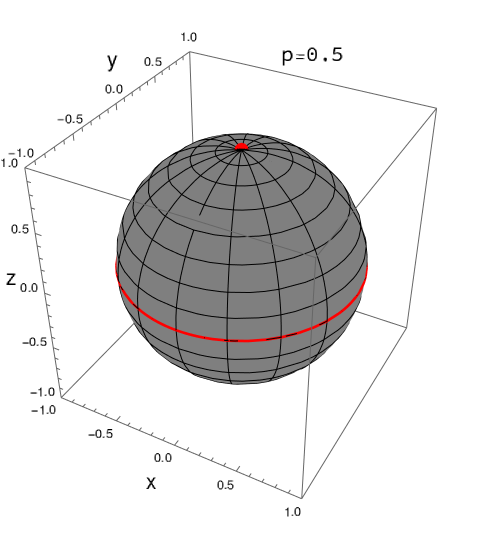
\includegraphics[width=0.9\linewidth]{chapter3/figures_special/sphere_Ising_t=0._z=0.9_p=0.5.png}
      \caption{$t=0$}
    \end{subfigure}%
    \begin{subfigure}{0.32\textwidth}
      \centering
      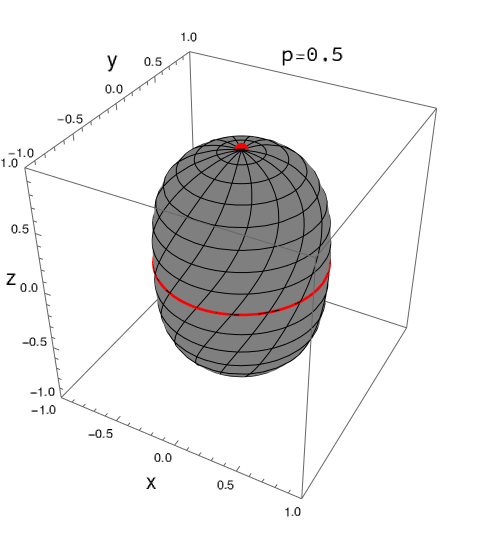
\includegraphics[width=0.9\linewidth]{chapter3/figures_special/sphere_Ising_t=0.5_z=0.9_p=0.5.png}
      \caption{$t=0.5$}
    \end{subfigure}
    \begin{subfigure}{0.32\textwidth}
      \centering
      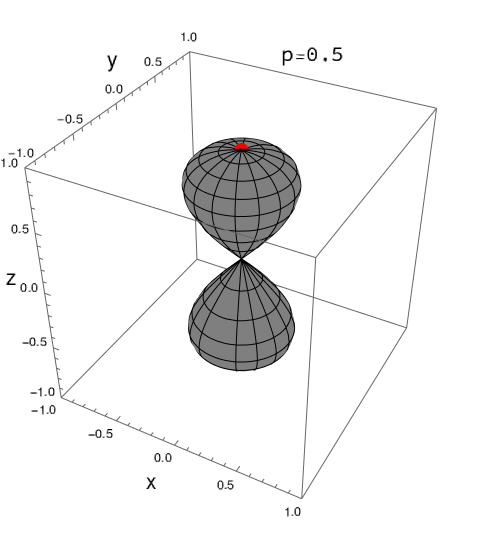
\includegraphics[width=0.9\linewidth]{chapter3/figures_special/sphere_Ising_t=1._z=0.9_p=0.5.png}
      \caption{$t=1$}
    \end{subfigure}
    \caption{Efecto del la evolución sobre la esfera de Bloch cuando $p=\frac{1}{2}$. Nótese que el desfasamiento sólo se completa en el eje $xy$.}
    \label{fig:Ising_p0.5_Sequence}
    \end{figure}

La despolarización dependiente de la componente en $z$ inicial es más clara si se observa el efecto de la evolución sobre el vector de Bloch. Abusando un poco de la notación se nota que 

\begin{equation*}
    \Gamma_{t}^{p=\frac{1}{2}}(\vec{r}_{\rho})=\begin{pmatrix}
        x\cos(2\omega t)-yz\sin(2\omega t)\\
        y\cos(2\omega t)+xz(2\omega t)\\
        z\\
    \end{pmatrix}
\end{equation*}
\acnote{Aquí se ve la casi rotación, pero creo que lo tengo que descomponer en diferentes operaciones para notar que el desfasamiento se da de forma más fuerte conforme más pequeño es z}
